\subsection{Movement Testing}
\label{subsec:movementtesting}

\begin{figure} [ht]
  \centering
  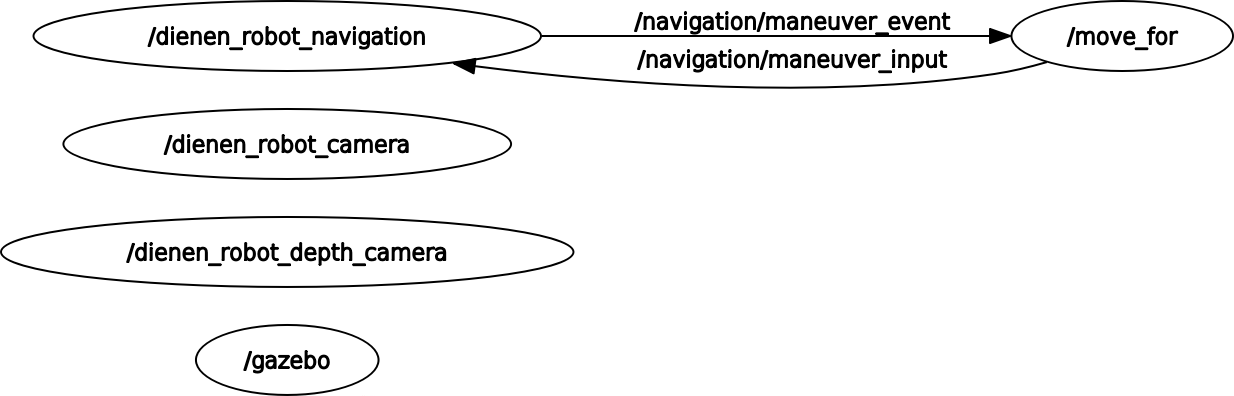
\includegraphics[width=0.45\textwidth]{figures/rosgraph/simulation-movement-test.png}
  \IfLanguageName{english}{
    \caption{Node scheme of the movement testing on the real robot.}
  }{
    \caption{Skema \emph{node} pengujian gerakan di simulasi.}
  }
  \label{fig:rosgraphrealrobotmovementtest}
\end{figure}

\begin{figure} [ht]
  \centering
  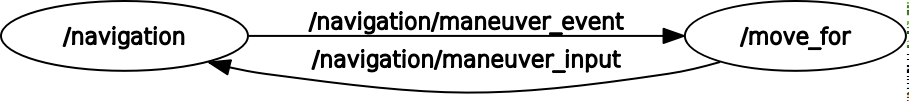
\includegraphics[width=0.45\textwidth]{figures/rosgraph/real-robot-movement-test.png}
  \IfLanguageName{english}{
    \caption{Node scheme of the movement testing in the simulation.}
  }{
    \caption{Skema \emph{node} pengujian gerakan pada robot fisik.}
  }
  \label{fig:rosgraphsimulationmovementtest}
\end{figure}


Movement testing is done by running the \lstinline{move_for} node as a behavior node that will instruct the robot to move at a certain speed for a certain period of time.
As shown in Figure \ref{fig:rosgraphsimulationmovementtest},
  in the simulation,
  the \lstinline{move_for} node will be connected to the \lstinline{dienen_robot_navigation} node to control the speed of the robot using the \lstinline{/navigation/maneuver_input} topic.
As for testing in the real world, as shown in Figure \ref{fig:rosgraphrealrobotmovementtest},
  the role of the \lstinline{dienen_robot_navigation} node which manages the navigation on the virtual robot will be replaced by the \lstinline{navigation} node which manages the navigation on the real robot.


\begin{figure}[ht]
  \centering
  \begin{tikzpicture}
    \begin{axis}[
        height=0.2\textwidth,
        width=0.45\textwidth,
        ylabel=\IfLanguageName{english}{Distance}{Jarak} (meter),xlabel=\IfLanguageName{english}{$K^{th}$ Attempt}{Percobaan Ke-$K$},
        legend style={
          at={(0.5,1.5)},
          anchor=north,
          legend columns=-1,
        },
        ymajorgrids,
        bar width=3pt,
        ybar=0pt,
        xmin=0.1,
        xmax=12.9,
        ymin=0,
        xtick distance=1,
        ytick distance=1,
      ]
      \addplot table[x=index,y=expecteddistance,col sep=comma]{data/linear-movement-sim.csv};
      \addplot table[x=index,y=measureddistance,col sep=comma]{data/linear-movement-sim.csv};
      \addplot table[x=index,y=odometrydistance,col sep=comma]{data/linear-movement-sim.csv};
      \IfLanguageName{english}{
        \legend{Estimated,Measurement,Odometry}
      }{
        \legend{Perkiraan,Pengukuran,Odometri}
      }
    \end{axis}
  \end{tikzpicture}
  \IfLanguageName{english}{
    \caption{Comparison of last distance results from the expected and measured values in the simulation.}
  }{
    \caption{Perbandingan hasil jarak akhir dari nilai yang diharapkan dan yang terukur di simulasi.}
  }
  \label{fig:linearmovementsim}
\end{figure}


\begin{figure}[ht]
  \centering
  \begin{tikzpicture}
    \begin{axis}[
        height=0.19\textwidth,
        width=0.45\textwidth,
        ylabel=\IfLanguageName{english}{Angle}{Sudut} (degree),xlabel=\IfLanguageName{english}{$K^{th}$ Attempt}{Percobaan Ke-$K$},
        legend style={
          at={(0.5,1.5)},
          anchor=north,
          legend columns=-1,
        },
        ymajorgrids,
        bar width=5pt,
        ybar=0pt,
        xmin=0.1,
        xmax=6.9,
        ymin=0,
        xtick distance=1,
        ytick distance=90,
      ]
      \addplot table[x=index,y=expected,col sep=comma]{data/angular-movement-sim.csv};
      \addplot table[x=index,y=measured,col sep=comma]{data/angular-movement-sim.csv};
      \addplot table[x=index,y=odometry,col sep=comma]{data/angular-movement-sim.csv};
      \IfLanguageName{english}{
        \legend{Estimated,Measurement,Odometry}
      }{
        \legend{Perkiraan,Pengukuran,Odometri}
      }
    \end{axis}
  \end{tikzpicture}
  \IfLanguageName{english}{
    \caption{Last orientation results of angular movement in the simulation.}
  }{
    \caption{Hasil orientasi akhir dari gerakan putar di simulasi.}
  }
  \label{fig:angularmovementsim}
\end{figure}


The movement test is divided into two parts,
  linear movement testing and angular movement testing,
  each is tested for 10 seconds on a virtual robot in a simulation environment and on a real robot in the real world.
As shown in Figure \ref{fig:linearmovementsim} and Figure \ref{fig:angularmovementsim},
  the position and orientation of the odometry received by the robot has the same value as the position and orientation of the robot model in the simulation.
This happens because the odometry value sent by the \lstinline{dienen_robot_navigation} node is the same value as the robot model transformation in the simulation.


\begin{figure}[ht]
  \centering
  \begin{tikzpicture}
    \begin{axis}[
        height=0.2\textwidth,
        width=0.45\textwidth,
        ylabel=\IfLanguageName{english}{Distance}{Jarak} (meter),
        xlabel=\IfLanguageName{english}{K Attempt}{Percobaan Ke-},
        legend style={
          at={(0.5,1.5)},
          anchor=north,
          legend columns=-1,
        },
        ymajorgrids,
        bar width=3pt,
        ybar=0pt,
        xmin=0.1,
        xmax=12.9,
        ymin=0,
        xtick distance=1,
        ytick distance=1,
      ]
      \addplot table[x=index,y=expecteddistance,col sep=comma]{data/linear-movement-real.csv};
      \addplot table[x=index,y=measureddistance,col sep=comma]{data/linear-movement-real.csv};
      \addplot table[x=index,y=odometrydistance,col sep=comma]{data/linear-movement-real.csv};
      \IfLanguageName{english}{
        \legend{Expected,Measured,Odometry}
      }{
        \legend{\emph{Expected},\emph{Measured},\emph{Odometry}}
      }
    \end{axis}
  \end{tikzpicture}
  \IfLanguageName{english}{
    \caption{Last distance results of linear movement in the real robot.}
  }{
    \caption{Hasil jarak akhir dari gerakan linier pada \emph{real robot}.}
  }
  \label{fig:linearmovementreal}
\end{figure}


\begin{figure}[ht]
  \centering
  \begin{tikzpicture}
    \begin{axis}[
        height=0.21\textwidth,
        width=0.45\textwidth,
        ylabel=\IfLanguageName{english}{Angle}{Sudut} (degree),
        xlabel=\IfLanguageName{english}{$K^{th}$ Attempt}{Percobaan Ke-$K$},
        legend style={
          at={(0.5,1.5)},
          anchor=north,
          legend columns=-1,
        },
        ymajorgrids,
        bar width=5pt,
        ybar=0pt,
        xmin=0.1,
        xmax=6.9,
        ymin=0,
        xtick distance=1,
        ytick distance=90,
      ]
      \addplot table[x=index,y=expected,col sep=comma]{data/angular-movement-real.csv};
      \addplot table[x=index,y=measured,col sep=comma]{data/angular-movement-real.csv};
      \addplot table[x=index,y=odometry,col sep=comma]{data/angular-movement-real.csv};
      \IfLanguageName{english}{
        \legend{Estimated,Measurement,Odometry}
      }{
        \legend{Perkiraan,Pengukuran,Odometri}
      }
    \end{axis}
  \end{tikzpicture}
  \IfLanguageName{english}{
    \caption{Last orientation results of angular movement on the real robot.}
  }{
    \caption{Hasil orientasi akhir dari gerakan putar pada robot fisik.}
  }
  \label{fig:angularmovementreal}
\end{figure}


In contrast to the movement testing in the simulation environment,
  movement testing in the real world have different results between direct measurements and the odometry values received by the robot.
As shown in Figure \ref{fig:linearmovementreal} and Figure \ref{fig:angularmovementreal},
  there is a difference between the two value due to inaccuracies in the sensors used to obtain position and orientation values.
However, despite the differences in the level of accuracy, by using the same node behavior,
  the robot is capable of carrying out appropriate movement commands when tested in the simulation and the real world.
